To numerically solve a set of PDEs, iterative methods are frequently used to approximate the solution by a step by step phenomena. Thus, the continuous time and space domains are discretized so that a set of numerical computations are iteratively (time discretization) applied on a mesh (space discretization). In other words, the PDEs are transformed to a set of numerical computations applied at each time step on all elements of the discretized space domain. Among the numerical computations is found a set of numerical schemes, also called \textit{stencil computations}.
A formal definition of a \textit{stencil program}, and the parallelization of such program, are presented in this section.

%-------------------------------------
\subsection{Definitions}

A mesh $\mathcal{M}$ defines the discretization of the continuous space domain $\Omega$ of a set of PDEs. 

\medskip
\begin{mydef}
\textit{A mesh is a connected undirected graph without bridges.}
\end{mydef}

$E_i$ denotes a set of elements constructed by a function $elem_i$ which defines a precise association of nodes and edges of a mesh. If we denote $nodes$ the function to get nodes of a mesh and $edges$ the same for edges, the funtion $elem_i$ is defined as
\begin{equation*}
elem_i : nodes(\mathcal{M}) \times edges(\mathcal{M}) \rightarrow E_i
\end{equation*}
For example, the set of cells $E_0$ in a Cartesian 2D mesh could be defined by exactly four nodes and four edges connected as a cycle. But we could also define another set of elements $E_1$ as the simple set of nodes etc.

A mesh can be structured (as Cartesian or curvilinear meshes), unstructured, regular or irregular (without the same topology for each element) and hybrid if mixing those. 

\begin{figure}[!h]\begin{center}
  \resizebox{8cm}{!}{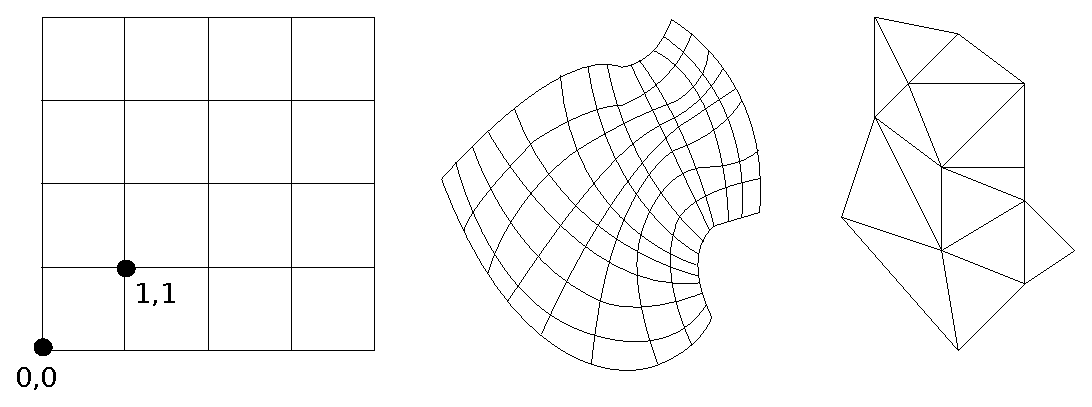
\includegraphics{./images/maillages.pdf}}
  \caption{From left to right, Cartesian, curvilinear and unstructured meshes.}
  \label{fig:mesh}
\end{center}\end{figure}

The discretization of the continuous time domain $\mathcal{T}$ is denoted $T$. $T$ is responsible for the iteration time steps of the numerical simulation. 

In a numerical simulation a set of data, or quantities, are applied onto the mesh and represent the set of values to compute, or to use, for computation. We denote the set of data applied on the mesh by $\Delta$, such that $\delta \in \Delta$ is a function which associates each element $el \in E_i$ to a value $v \in V$, 
\begin{equation*}
\delta : E_i \rightarrow V
\end{equation*}
One can notice that in applied mathematics, the signature of $\delta$ would be $\delta : E_i \times T \rightarrow V$, however when programming a numerical simulation it is not wise to store all values of each time iteration.

Finally, in a numerical simulation are performed a set of ordered numerical computations denoted $\Gamma$. A numerical computation in $\Gamma$ is denoted 
\begin{equation*}
c(R,w,D,e). 
\end{equation*}
In this definition $R \subset \Delta, w \in \Delta$ are respectively the data read and written to compute the numerical expression $e$ (a single data is written in a single computation). $D$ is one of the subsets $E_i \subset \mathcal{M}$. It has to be noticed that at each time iteration, all the elements of a mesh are computed. However, it happens that the computation of the mesh elements is splitted in different computations (for example the computation of the physical border). In this case additional $E_i$ can be specified for the mesh $\mathcal{M}$.
The numerical expression $e$ computes the data $w$ from a set of data $R$.
\begin{equation*}
e : R \rightarrow w
\end{equation*}

A \textit{multi-stencil program} is defined by the quadruplet
\begin{equation}
\mathcal{MSP}(T,\mathcal{M},\Delta,\Gamma),
\end{equation}

If the number of computations in $\Gamma$ is $card(\Gamma)=m$, such that $\bigcup_{i=0}^{m-1}c_i = \Gamma$, then $\bigcup_{i=0}^{m-1}R_i \cup w_i \subseteq \Delta$.

A computation $c \in \Gamma$ can be of two different types. The first type is called a \textit{stencil computation} and involves an additional information denoted $\mathcal{N}$ which represents a neighborhood function around an element
\begin{equation}
\mathcal{N} : E_i \rightarrow E_k \times E_k \times ...
\end{equation}
, where $E_k$ is a set of elements of $\mathcal{M}$ which could be equal to $E_i$ or not. In other words, from an element $el \in E_i$ the function $\mathcal{N}$ returns a set of elements of $E_k$ which represents the neighborhood of $el$. The function $\mathcal{N}$ is also sometimes called the \textit{stencil shape}, or the \textit{stencil} in applied mathematics.

A \textit{stencil computation} is a quintuplet
\begin{equation}
s(R,w,D,e,\mathcal{N}),
\end{equation}
where $R \subset \Delta, w \in \Delta$ are read and written in the numerical expression $e$, and $D$ is one the subsets $E_i$. In a stencil computation $s$, $\forall d \in D$, the stencil numerical expression $e$ is applied such that $w(d) = e(R(d),R(\mathcal{N}(d))$. In this work, a stencil computation $s(R,w,D,e,\mathcal{N})$ always verifies $R \cap w = \emptyset$, otherwize an implicit numerical scheme has to be solve which is over the scope of this paper.

Figure~\ref{} gives an example of a stencil computation $s(R,w,D,e,\mathcal{N})$, on a two dimensional Cartesian mesh, where $R=\{A,B\}$, $w=C$, and where for $(x,y) \in D$
\begin{equation*}
e(R(x,y),R(\mathcal{N}(x,y)) = A(x,y)+B(x,y+1)+B(x,y-1)+B(x+1,y)+B(x-1,y).
\end{equation*}

Finally, the second type of numerical computation is a local computation where $e$ does not involve a neighborhood function $\mathcal{N}$
\begin{equation}
l(R,w,D,e)
\end{equation}

%-------------------------------------
\subsection{Parallelization}
\label{sect:parall}
% Multi-stencil mesh-based numerical simulation can be parallelized in various ways and is an interesting kind of application to take advantage of modern heterogeneous HPC architectures, mixing clusters, multi-cores CPUs, vectorization units, GPGPU and many-core accelerators.

% Maybe the more important parallelization technique of such simulations is called \textit{SPMD} (Single Program, Multiple Data) which can also be called \textit{coarse-grain data parallelism}. This concept represents the well-known and broadly-used domain decomposition technique to split the mesh in balanced sub-meshes for available resources. Because of the good locality degree of numerical simulations, only a small number of additional elements, called a \textit{recorvery} or a \textit{ghost} area, are needed to exchange information computed by another resource to correctly compute stencils. As the amount of communications of such parallelization are rather small compared to the amount of computations (small neighborhood), and also by the addition of recovery of communications by computations, this parallelization technique has proved many times its efficiency and scalability on numerical simulations~\cite{}. This parallelization technique can be applied on shared and distributed memory architectures (clusters, multi-core CPUs), and it stays the most efficient parallelization technique if the numerical simulation has to be executed on a distributed memory architecture. For this reason, this parallelization stays a reference in the domain and is still studied for more complex simulations, using unstructured meshes, multi-grids techniques etc.

% However, because of energy consumption constraints, most of the \textit{top500}~\footnote{http://www.top500.org} supercomputer centers are not only composed of clusters of multi-core machines, but also of accelerator cards such as GPGPU and many-cores. In addition to this, vectorization units are also available on most CPUs. This introduces another kind of parallelization, linked to the first one, called in this paper \textit{fine-grain data parallelism}, which is composed of \textit{SIMD} (Single Instruction, Multiple Data) and \textit{SIMT} (Single Instruction, Multiple Threads) parallelization techniques. Such techniques typically compute a numerical expression in parallel on a vector, using vectorization units or threads, which perfectly matches the type of computation in the nested loops of numerical simulations.

% Finally, the last parallelization technique which can be applied on various architectures (clusters, multi-cores, many-cores, GPGPU), is the \textit{task parallelism} technique. Instead of spliting the data of the simulation (or the vector used in a numerical expression), the different tasks of the simulation are identified and scheduled over the available resources during the execution (at runtime)~\cite{}. As numerical computations of a simulation can be considered as tasks, linked together through data dependencies for example, this parallelization technique can be used for HPC numerical simulations too.

% This section discussed the various parallelization techniques which can be used for numerical simulations. As a result, it seems that, by a combination of existing techniques, modern heterogeneous parallel architectures can be fully harnessed by such applications~\cite{}. In this paper is presented a component-based model to expose those three kinds of parallelism in the overall simulation, while hiding them from the user (numericians).

% %-------------------------------------
% \subsection{Dependencies and synchronizations}
% \label{sect:dep}
% To define and explain the component-based implicit parallelism model presented in this paper, two additional definitions handle the relations between data read and written into computations. Those relations are responsible for dependencies and synchronizations.

% \medskip
% \begin{mydef}
% \textit{For two computations $c_1(R_1,w_1,D_1,e_1)$ and $c_2(R_2,w_2,D_2,e_2)$, it is said that $c_2$ is dependant from $c_1$, denoted $c_1<c_2$, if $w_1 \cap R_2 \neq \emptyset$. In this case, $c_1$ has to be computed before $c_2$. The binary relation $c_1<c_2$ represents a \textit{dependency}.}
% \end{mydef}

% \medskip
% Dependencies lead to one computation before another, but when the program is parallelized some dependencies are also responsible for synchronizations between different processes. The opposite definition can also be given, 

% \medskip
% \begin{mydef}
% \textit{For two computations $c_1(R_1,w_1,D_1,e_1)$ and $c_2(R_2,w_2,D_2,e_2)$, it is said that $c_2$ is independant from $c_1$, denoted $c_1 \not <c_2$ or $c_1 \parallel c_2$, if $w_1 \cap R_2 = \emptyset$.}
% \end{mydef}

% Considering a coarse-grain data parallelized multi-stencil program $\mathcal{MSP}$,

% \medskip
% \begin{mydef}
% \textit{A depedency between two computations $c_1<c_2$ is a \textit{synchronisation}, denoted $c_1 \ll c_2$, if $c_2=s_2(R_2,w_2,D_2,e_2)$, and $w_1 \cap R_2 \neq \emptyset$.}
% \end{mydef}

% \medskip
% Actually, in a parallel stencil program, synchronizations between processes are always needed for the set of data $R$ of a stencil $s(R,w,D,e)$ because the expression $e$ involves a neighborhood $\mathcal{N}$ which could be handled by another processor or resource.


